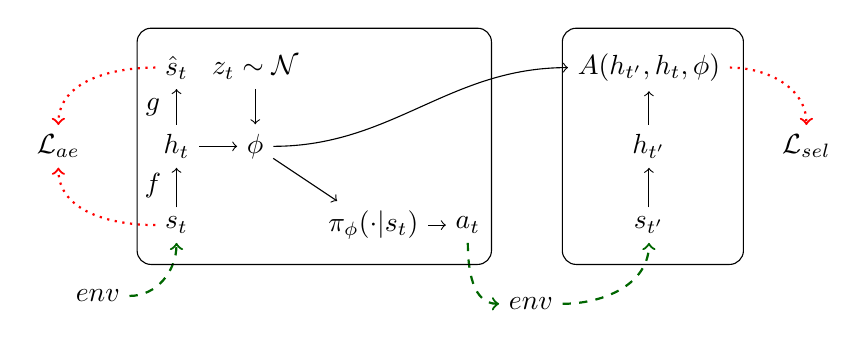
\begin{tikzpicture}

\def \pA {0}
\def \pB {6}
\def \pmid {2.5}

\node[] (st) at (\pA,0) {$s_t$};
\node[] (ht) at (\pA,1) {$h_t$};
\node (st_rec) at (\pA,2) {$\hat{s}_t$};

\draw[->,draw=black] (st) to (ht);
\draw[->,draw=black] (ht) to (st_rec);
\node at (-.3,1.5) {$g$};
\node at (-.3,0.5) {$f$};

\node (env) at (-1,-0.9) {$env$};
\draw[->,draw=black!60!green,dashed,thick] (env) to[out=0,in=-90] (st);


\node[] (st1) at (\pB,0) {$s_{t'}$};
\node[] (ht1) at (\pB,1) {$h_{t'}$};
\draw[->,draw=black] (st1) to (ht1);

\node[] (pi0) at (\pmid,0) {$\pi_\phi(\cdot|s_t)$};
\node[] (phi0) at (\pmid-1.5,1) {$\phi$};
\node[] (z0) at (\pmid-1.5,2) {$z_t \sim \mathcal{N}$};
\node[] (A1) at (\pB,2) {$A(h_{t'}, h_t,\phi)$};
\draw[->,draw=black] (z0) to (phi0);
\draw[->,draw=black] (ht) to (phi0);
\draw[->,draw=black] (phi0) to (pi0);
\draw[->,draw=black] (phi0) to[in=180,out=0] (A1);
\draw[->,draw=black] (ht1) to (A1);

\begin{scope}[]

\end{scope}
\node[] (aT) at (\pmid+1.2,-0) {$a_t$};
\node[] (env1) at (\pmid+2,-1) {$env$};
\draw[->] (pi0) to (aT);
\draw[->,draw=black!60!green,dashed,thick] (aT) to[out=-90,in=180] (env1);
\draw[->,draw=black!60!green,dashed,thick] (env1) to[out=0,in=-90] (st1);

\node[] (lossAE) at (\pA-1.5,1) {$\mathcal{L}_{ae}$};
\draw[->,draw=red,dotted,thick] (st) to[out=180,in=-90] (lossAE);
\draw[->,draw=red,dotted,thick] (st_rec) to[out=180,in=90] (lossAE);

\node[] (lossSel) at (\pB+2,1) {$\mathcal{L}_{sel}$};
\draw[->,draw=red,dotted,thick] (A1) to[out=0,in=90] (lossSel);

\draw
  {[rounded corners=5pt](-0.5,-0.5)  --
  (\pmid+1.5,-0.5)  -- 
  (\pmid+1.5,2.5) --
  (-0.5,2.5) --
  cycle};
\draw
  {[rounded corners=5pt](-1.1+\pB,-0.5)  --
  (1.2+\pB,-0.5)  -- 
  (1.2+\pB,2.5) --
  (-1.1+\pB,2.5) --
  cycle};
\end{tikzpicture}